\subsection{Introduction}\label{subsec:2.3.data_synth_intro}
%The process of training AI models heavily relies on the quality of the datasets involved, including the quality of the samples, the quality of the annotations, and the amount of samples among other factors. Whilst the MANOLO data quality assessment module, addressed in the previous task in this workpackage, assesses data quality, an overall lack of data during training often leads to bias in model predictions as well as poor model performance at inference time. 

%The MANOLO submodule discussed in this section, the Data and Feature Synthetisation submodule, compiles a set of techniques to generate synthetic data in the form of new unseen samples or their equivalent extracted features. This allows the user to address the challenges stemming from a lack of data, whether increasing the overall number of training examples to increase data variability, generating data from a particular class to address class imbalance, or directly mitigating biasses in the dataset. 

%The first version of the deliverable reports the efforts undertaken towards data synthetisation through the experimentation with Invertible Neural Networks. These networks are trained on classification datasets, then, they can generate a new sample compatible with a given label, according to the learned parameters of the network. Section~\ref{subsec:2.3_datasynth_tech1} introduces the technique as it will be part of the MANOLO library, in the conditional version (cINNs). The initial cINNs implementation for the MANOLO data module allows the generation of samples from a dataset and the generative condition extends from a particular class to a style contained in the latent space.

AI practitioners training models for classification, forecasting, or more complex tasks usually find that their datasets lack balance in the representation that certain attributes or classes have, which can cause biases during inference time, or affect the robustness of the models. Thus, MANOLO will provide tools to generate synthetic data, or synthetic features (following the philosophy of the previous section), to make sure that the model training and optimization phase increases its trustworthiness in another additional manner.

Data synthesis approaches can be grouped in two main categories: knowledge based and model based approaches. Knowledge based approaches utilize traditional engineering approaches and require the expert knowledge of humans to design strategies to generate new samples~\citep{2015_NeurIPS_character, 2021_arxiv_AEDA, 2021_arxiv_data}. These approaches are time consuming, require human intervention and are usually limited to certain domains and tasks. Model based approaches use trained models that are wether trained in the target dataset for the specific domain of the target application~\citep{2014_NeurIPS_GAN, 2016_ACL_improving, 2019_arxiv_cinn}, or trained on large datasets that often combine multiple modalities~\citep{2024_WACV_Semantic, 2024_CVPR_towards, 2024_ICASP_image}. The model based approaches outperform the knowledge based in data generation: provides more variety, higher sample quality, and less human intervention required. Note that the computational costs of this approaches is overall higher and increases as model size increases.  

At the time of this deliverable, this section presents two initial frameworks for conditional sample generation that will be include in the Data Generation MANOLO submodule: invertible neural networks and generative adversarial networks. For a better evaluation of these frameworks, this section currently focuses on image datasets. The first framework introduced in this deliverable, invertible neural networks, is an efficient solution to data generation that provides a considerable degree of freedom in the conditioning stage allowing the user to alter the class and style of the selected samples. The second framework, generative adversarial networks, provides additional versatility in the selection of model architecture, which facilitates the scalability of the models to larger datasets and different modalities.

%%%%%%%%%%%%%%%% Conditional Invertible Neural Networks  %%%%%%%%%%%%%%%%
\subsection{Conditional INNs}
\label{subsec:2.3_datasynth_tech1}

Ideally, it would be very convenient to train a simple classification NN model with a given dataset and then input a label (previously the target) so as to generate a new data sample (previously the input). Unfortunately, NNs are not invertible by definition, and need to be designed for this specific purpose. This is where Invertible Neural Networks enter. These NNs, bijective by definition, have a constrained set of possible layers, which exclude batch normalization and pooling, for instance, and allow the generation of samples from a desired label. We take a step forward with the use of Conditional Invertible Neural Networks (CINNs), a variation of invertible neural networks that provides the possibility of selecting the class of the generated sample. Additionally we include a methodology to furhter condition the sample generation stage and allow the user to tweak the style of the generated samples. In this subsection we address data generation with the conditional invertible neural networks proposed by Ardizonne et al.~\cite{2019_arxiv_cinn}. 

When conditional generation is introduced, INNs are trained to map an input sample to a latent space while being conditioned by the class of the sample. Then, at inference time, the inverted model can be used as a unit that processes random vectors from the latent space and produces unseen samples in the input space. This inversion procedure is conditioned by the sample class to constrain the generation to a particular class. In the case of computer vision, for instance, INNs map an image from the image space (RGB representation) to a latent vector. This deliverable will show an initial exploration of class and style conditioning alternatives. These approaches allow the model to generate class conditioned images with a particular style living in the latent space.

        
\subsubsection{Methodology}

This subsection describes the technical aspects of the approach introduced in this version of the deliverable: the CINN proposed by~\cite{2019_arxiv_cinn}. This approach uses linear neural networks and conditions the sample generation with class labels. This subsection also includes the adaptation we proposed to condition the style of the generated samples, and a description of the experimental setup used to obtain the results reported in the following subsection.

\subsubsection*{Class-conditioned sample generation.} 
\begin{quote}
Sample generation with INNs, as with normalising flows~\cite{2018_NeurIPS_GLOW}, is based on the principle behind the change of variable statistics formula 
% 
\begin{equation}
p_{X}(X) = p_{Z}(f(X))|\det Df(X)|^{-1},     
\end{equation}
% 
where $p_{X}(X)$ and $p_{Z}(f(X))$ are the probability distributions from the input and the latent space respectively, $\det Df(X)$ is the determinant of the Jacobian of $f(X)$, and $f(X)$ is the model or mapping function that is going to be learned. We train this model, as is most commonly done, via maximum likelihood. Following the mathematical developments by Ardizonne et al.~\cite{2019_arxiv_cinn}, which include the prior conditioning of the model with the class of the input sample, this results in the minimization of three terms: the squared module of the model prediction, the logarithm of the Jacobian of the model weights, and a regularization to enforce a Gaussian space being learned.

Class-conditioned sample generation relies on a prior introduced during training and inference that alters the mapping and constricts it to a particular region of the latent space, the region that belongs to the samples under the given condition. The prior used for class-conditional sample generation consist of a one-hot-encoded vector representing the semantic class of a sample. This is shown in Figure~\ref{fig:class_conditional_generation}, where the input $z_i$ is a random Gaussian noise vector, the condition $c_i$ is a vector indicating the class ``3'' in this particular example, and $x_i$, in this case the output of the inverted model, is a newly generated image of a digit ``3''. By using different noise vectors as seeds for the generation of samples, the model outputs different new samples all corresponding to the category indicated by the condition vector. 

\begin{figure}[h]
    % \vskip -0.2in 
    \centering
    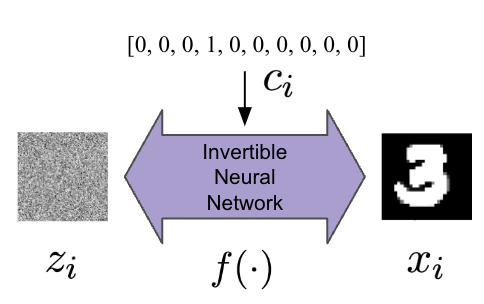
\includegraphics[width=0.40\columnwidth]{fig_datasynth/class_conditional_generation.png} 
    \caption[Class-conditional sample generation]{\label{fig:class_conditional_generation} The invertible neural network $f(\cdot)$ generates an unseen sample $x_i$ from a Gaussian noise vector $z_i$ given a class condition $c_i$ and vice-versa.} 
    % \vskip -0.2in 
    % \vspace{-2pt}
    % \caption{\label{fig:class_conditional_generation} The invertible neural network $f(\cdot)$ generates an unseen sample $x_i$ from a Gaussian noise vector $z_i$ given a class condition $c_i$ and vice-versa.}
    % \vskip -0.0in 
\end{figure}

\end{quote}

\subsubsection*{Style-and-class-conditioned sample generation} 

\begin{quote}
Style-and-class-conditioned sample generation goes a step farther, assumes that the class condition is fixed, and conditions the sample generation to adhere to a particular style. We define the style by exploring the latent space learned by the CINN and select a set of seed noise vectors near the area of interest, i.e. the noise vectors corresponding to a set of samples that exhibit the style in which we are interested. Since different latent vectors result in different images being generated, by moving a random noise vector towards a region in the latent space where a particular set of samples belong, we condition the generation of samples. This is depicted Figure~\ref{fig:ciinn_style_conditioning}. 

To define the region of the latent space that contains the style we want, we define a style vector $z_s$ that represents the style we are interested in. We do this by manually selecting $K$ samples that share the particular style we want (bold, italic, faint writing in the MNIST example) and mapping them to the latent space, resulting in a latent style vector per sample $\{z_{s1}, z_{s2}, ..., z_{sK}\}$. Then we define the style vector as the centroid of the individual style vectors 
% 
\begin{equation}
    z_{s} = 1/K \sum_{i} z_{si}.
\end{equation}
% 
Finally, we generate samples using the interpolation of $z_{s}$ with a random Gaussian noise vector $z_i$ as a conditioned seed vector 
% 
\begin{equation}
    z_c = (1-t) z_i + t z_{s} 
\end{equation}
% 
that falls close to a region in the latent space that encodes a particular style. Figure~\ref{fig:ciinn_style_conditioning} illustrates this process with the ``bold'' style for the MNIST dataset. The strength of the interpolation modulates how close the $z_c$ vector is to the style vector $z_s$ and, consequently, how strong will the presence of the particular style be in the generated image.
\end{quote}


\begin{figure}
    % \vskip -0.2in 
    \centering
    \vspace{-2pt}
    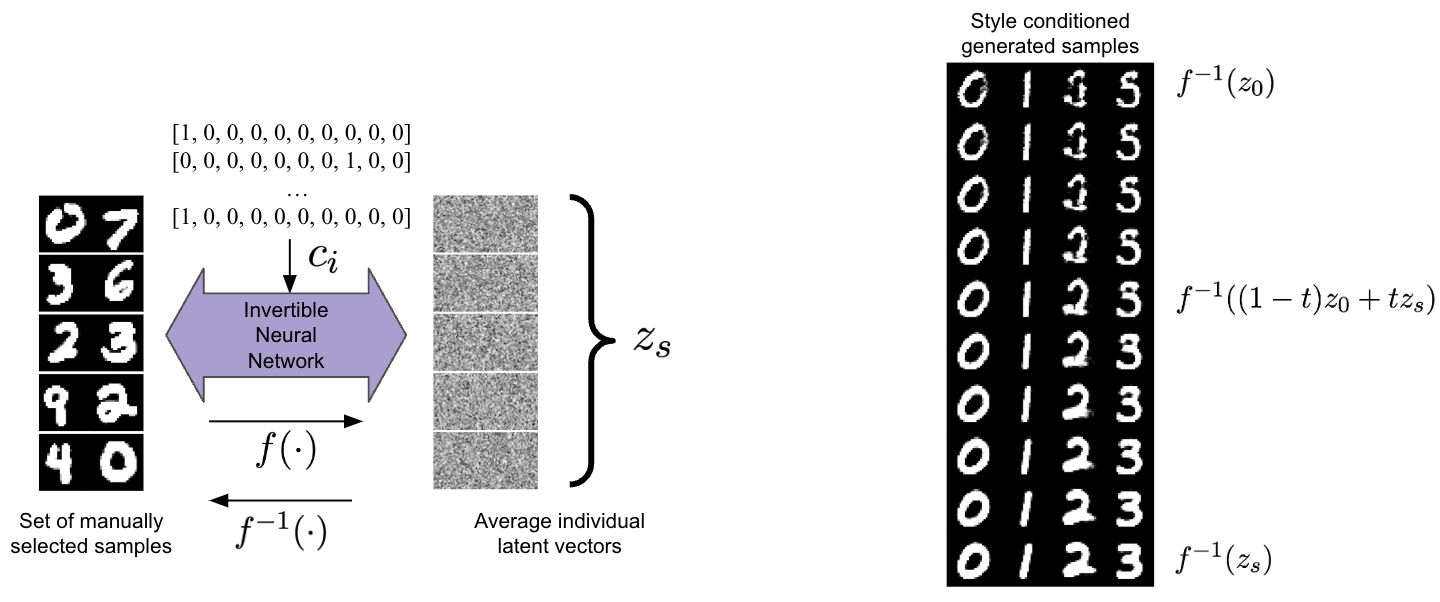
\includegraphics[width=1.0\columnwidth]{fig_datasynth/style_conditional_generation.png} 
    \caption[Style-conditioned sample generation]{\label{fig:ciinn_style_conditioning} The latent vectors of a manually selected set of samples are averaged to create the latent vector $z_S$ that defines the style (left). Through a weighted average of the style vector and the seed random vector, the CINN regulates the strengths of the style-conditioning (right).}
    % \vspace{-2pt}
    % \caption{\label{fig:ciinn_style_conditioning} The latent vectors of a manually selected set of samples are averaged to create the latent vector $z_S$ that defines the style (left). Through a weighted average of the style vector and teh seed random vector, the CINN regulates the strengths of the style-conditioning (right).}
    % \vskip -0.0in 
\end{figure}




\subsubsection*{Experimental setup} 
\begin{quote}
The sample generation functionality for the Data Inspection and Generation MANOLO submodule is currently developed and tested on the MNIST~\cite{1998_IEEE_MNIST} and Fashion-MNIST~\cite{2017fashionMNIST}. These are two small datasets, widely used in the research community that allow for faster experiemtnation. MNIST contains 60,000 black and white 28$\times$28 images of hand-written digits group into ten different classes corresponding to the digits 0-9. Fashion-MNIST is a more challenging dataset with very similar characteristics: black and white 28$\times$28 images, 60,000 for training and 10,000 for testing, distributed across 10 classes that belong to the retail domain each containing one clothing item.  
    
The experiments presented in this section use the CINN model  proposed in~\cite{2019_arxiv_cinn}, composed of 20 linear layers as implemented in the FrEIA library~\cite{freia}. Hence, the images are flattened into a 784 dimensional vector in the input of the model and then unflattened back at the output. The INN is trained on 256 samples batches with Adam optimizer and a learning rate of $10^{-5}$ that we reduced by a factor of 10 at epoch 20 and epoch 40 of a 60 epochs training.
\end{quote}


\subsubsection{Results}

\subsubsection*{Class-conditioned sample generation} 
\begin{quote}
The experiments on class-conditional sample generation illustrate the ability of a CINN to generate samples from a given class.  Figure~\ref{fig:exp_class_cond_MNIST} and~\ref{fig:exp_class_cond_FashionMNIST} provide examples of images generated by a CINN for each class in the MNIST and Fashion-MNIST dataset respectively. 
\end{quote}

\begin{figure}[h]
    % \vskip -0.1in 
    \centering
    \caption{\label{fig:exp_class_cond_MNIST} Samples generated by the CINN for each of the ten classes in the MNIST dataset.}
    \vspace{-0.15in}
    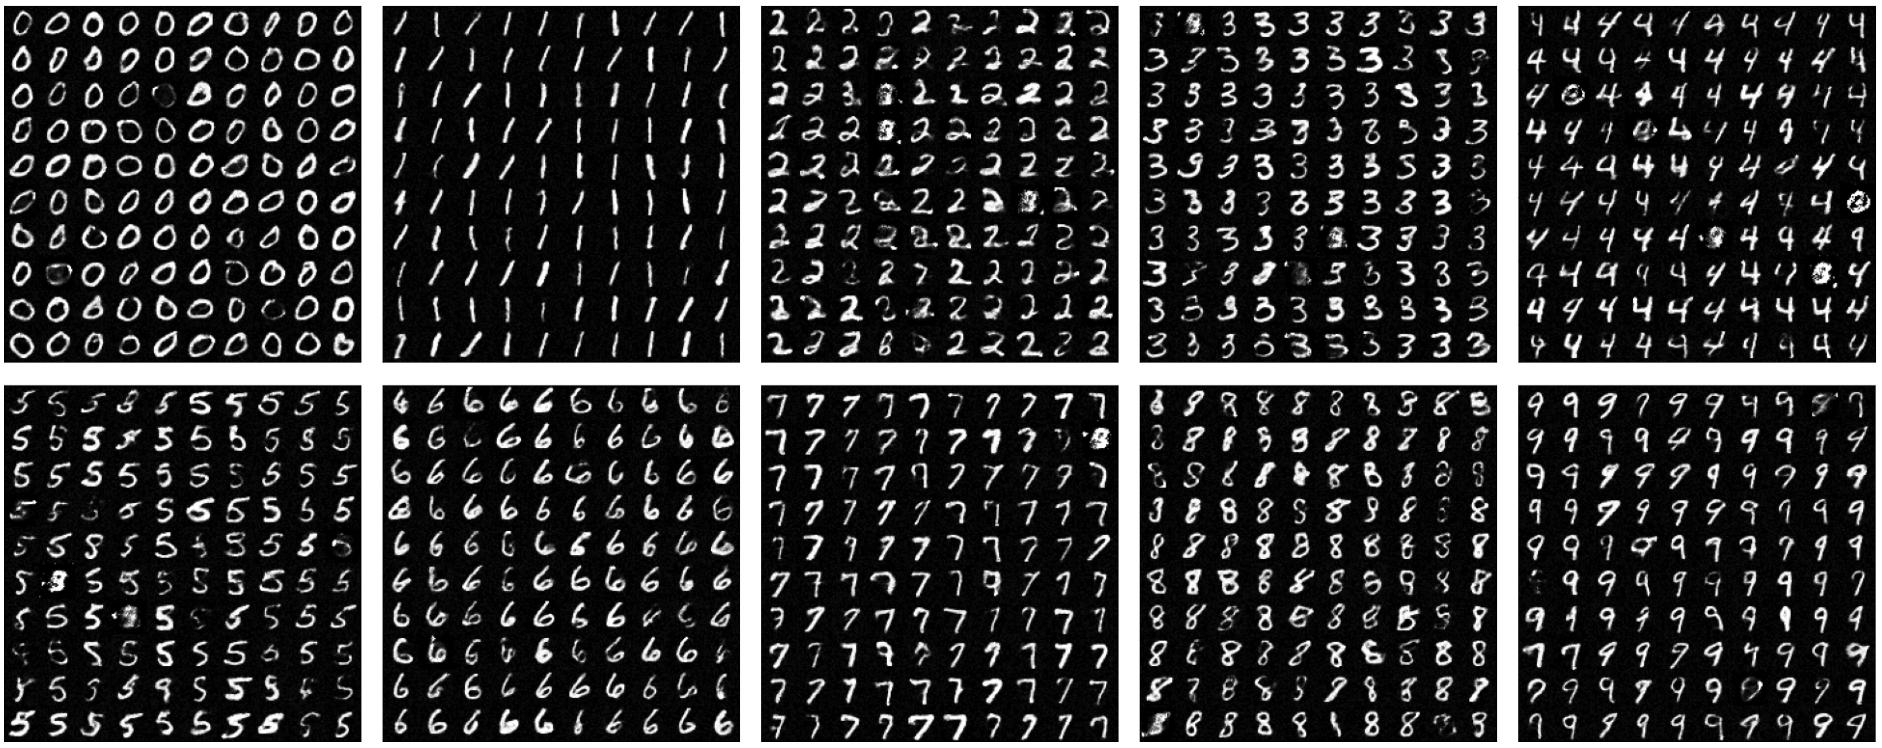
\includegraphics[width=0.95\columnwidth]{fig_datasynth/class_conditional_generation_MNIST.png} 
    % \vspace{-0.15in}
    % \caption{\label{fig:exp_class_cond_MNIST} Samples generated by the CINN for each of the ten classes in the MNIST dataset.}
    % \vskip -0.0in 
\end{figure}

\begin{figure}[h]
    % \vskip -0.1in 
    \centering
    \caption{\label{fig:exp_class_cond_FashionMNIST} Samples generated by the CINN for each of the ten classes in the Fashion-MNIST dataset.}
    \vspace{-0.15in}
    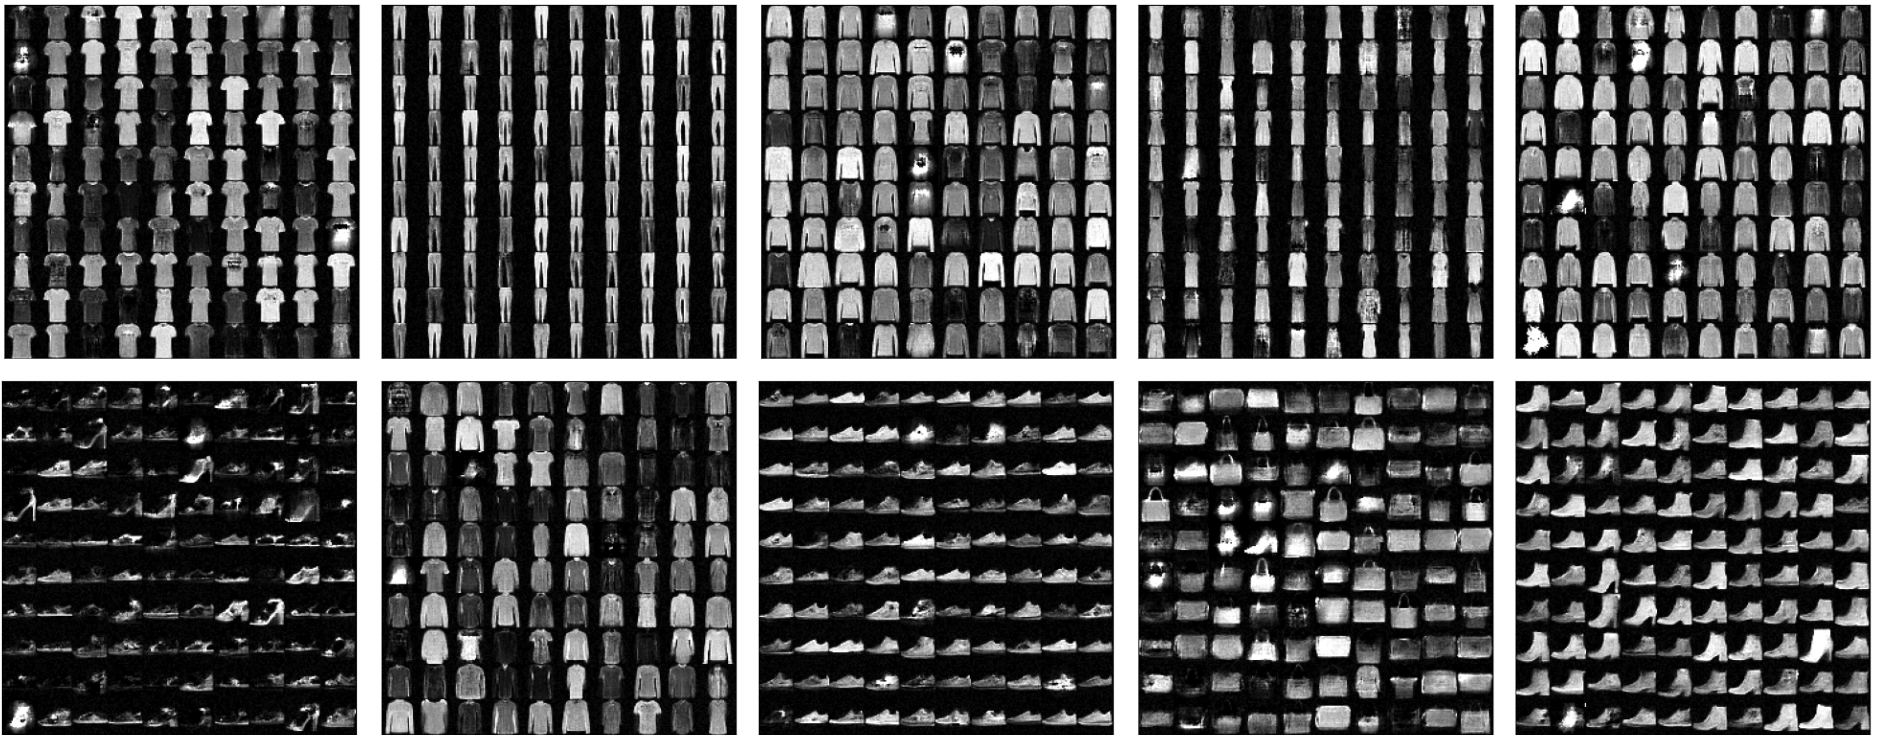
\includegraphics[width=0.95\columnwidth]{fig_datasynth/class_conditional_generation_Fashion-MNIST.png}     
    % \vspace{-0.15in}
    % \caption{\label{fig:exp_class_cond_FashionMNIST} Samples generated by the CINN for each of the ten classes in the Fashion-MNIST dataset.}
    % \vskip -0.0in 
\end{figure}    


\subsubsection*{Style-and-class-conditioned generation.} 
\begin{quote}
The results in this section demonstrate how we further condition the sample generation process to enforce a particular style in the generated samples. Figures~\ref{fig:bold_conditioned_generated_samples} and~\ref{fig:italic_conditioned_generated_samples}, provide examples of style-and-class conditioned generated samples and the corresponding initial seeds used for the MNIST dataset. Similarly, Figure~\ref{fig:striped_conditioned_generated_samples} provide the generated samples for Fashion-MNIST, in this case we only use a single image to define the style due to the large variety in styles present in the dataset. These figures help illustrate the generation process: the left side of the figures contain samples manually selected that belong to a particular style, bold and italic for MNIST and striped for Fashion-MNIST. Then, the images to the right of the figures correspond to the samples generated for the ten different class conditions (digits from zero to nine in MNIST and the different retail categories in Fashion-MNIST), and each row from top to bottom, correspond to an increasing level of style conditioning strength. The top row samples are generated from a completely random seed vector, the bottom row samples from the style vector obtained from the manually selected samples, and the rows in between interpolations of these vectors. The strength of the interpolation, and of the conditioning consequently, is defined by a parameter $t$ and in these results is linearly and increased between zero and one. 
\end{quote}

\begin{figure}[h!]
    \vskip -0.1in 
    \centering
    \caption{\label{fig:bold_conditioned_generated_samples} Style-and-class-conditioned samples for the bold style in the MNIST dataset.}
    \vspace{-0.1in}
    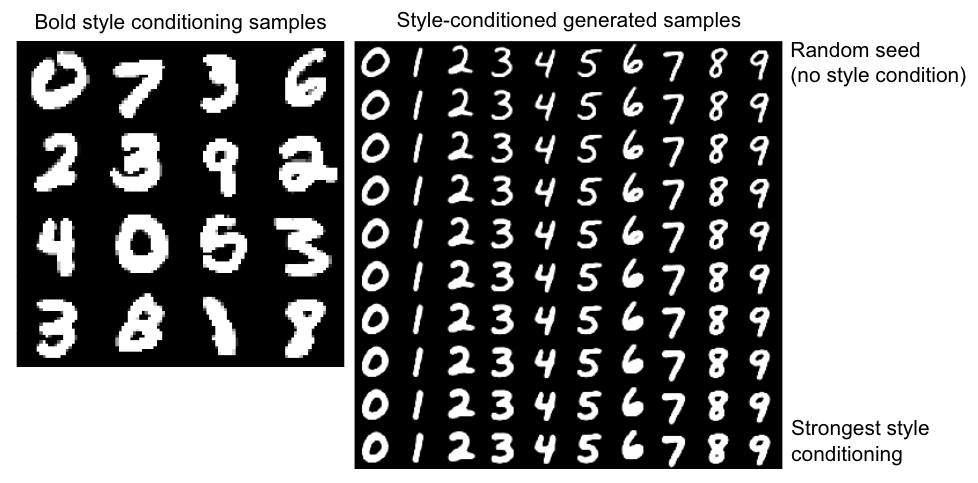
\includegraphics[width=0.78\columnwidth]{fig_datasynth/bold_conditioned_generated_samples.png} 
    % \vspace{-0.2in}
    % \caption{\label{fig:bold_conditioned_generated_samples} Style-and-class-conditioned samples for the bold style in the MNIST dataset.}
    % \vskip -0.0in 
\end{figure}

\begin{figure}[h!]
    \vskip -0.1in 
    \centering
    \caption{\label{fig:italic_conditioned_generated_samples} Style-and-class-conditioned samples for the italic style in the MNIST dataset.}
    \vspace{-0.1in}
    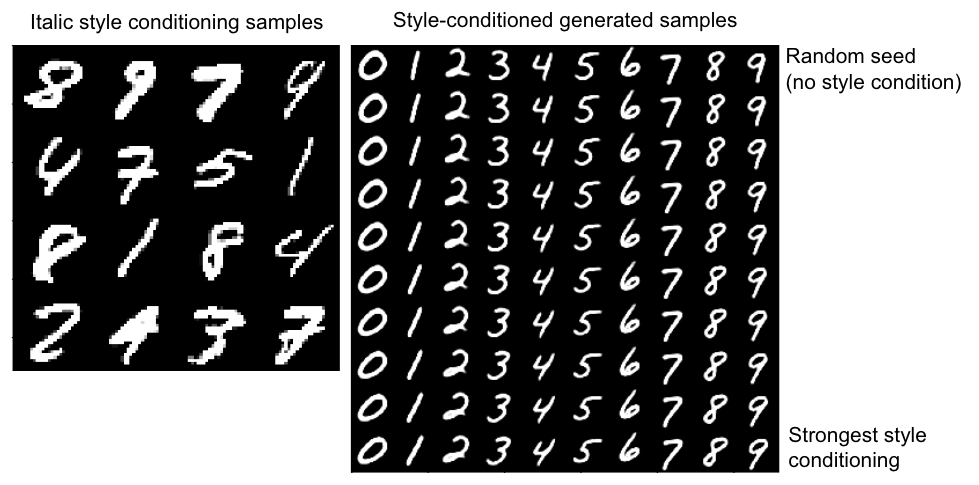
\includegraphics[width=0.78\columnwidth]{fig_datasynth/italic_conditioned_generated_samples.png} 
    % \vspace{-0.2in}
    % \caption{\label{fig:italic_conditioned_generated_samples} Style-and-class-conditioned samples for the italic style in the MNIST dataset.}
    % \vskip -0.0in 
\end{figure}

\begin{figure}[h!]
    \vskip -0.1in 
    \centering
    \caption{\label{fig:striped_conditioned_generated_samples} Style-and-class-conditioned samples for the striped style in the Fashion-MNIST dataset.}
    \vspace{-0.1in}
    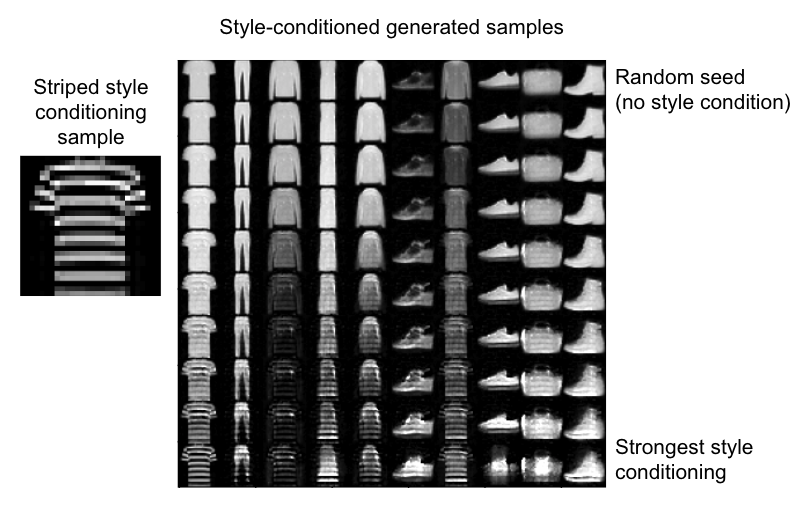
\includegraphics[width=0.78\columnwidth]{fig_datasynth/striped_conditioned_generated_samples.png} 
    % \vspace{-0.2in}
    % \caption{\label{fig:striped_conditioned_generated_samples} Style-and-class-conditioned samples for the striped style in the Fashion-MNIST dataset.}
    % \vskip -0.0in 
\end{figure}



%%%%%%%%%%%%%%%% GANs %%%%%%%%%%%%%%%%
\subsection{Generative Adversarial Networks}
\label{subsec:2.3_datasynth_tech2}

Data generation requires custom models to address different datasets and domains, which is particularly challenging when models are restricted to a limited number of architectures, as is the case in invertible neural networks~\ref{subsec:2.3_datasynth_tech1}. As a solution to this challenge and given their high quality results, Generative Adversarial Networks (GANs)~\citep{2014_NeurIPS_GAN} have become widely adopted by the machine learning community. These models provide a versatile framework that accommodates a wide range of  architectures allowing for a broader applicability. Additionally, the strategy used when training GANs require relatively low computational resources. Note that, while GANs are successful in generating images, they do not inherently present the style conditioning capabilities that other models do (see Section~\ref{subsec:2.3_datasynth_tech1}).

The GAN framework presented in this section is constituted of two neural networks, a generator and a discriminator, that are trained in an adversarial fashion: the generator is optimized to generate realistic samples and the discriminator to distinguish between real and generated samples. This creates a competition between models that forces them to improve without external supervision. As illustrated in Figure~\ref{fig:gans_schematic}, the training process iterates between two stages: in the first stage the discriminator's parameters are optimized to better identify the fake or generated images and in the second stage the generator's parameters are optimized to outsmart the discriminator by making samples that look as real as possible.  

\begin{figure}[h]
    % \vskip -0.2in 
    \centering
    \caption[GAN training framework.]{\label{fig:gans_schematic} GAN training framework. In stage one (top) the discriminator is trained and in stage two (bottom) the generator is trained. Blue color is used to represent the blocks being trained in each stage.}
    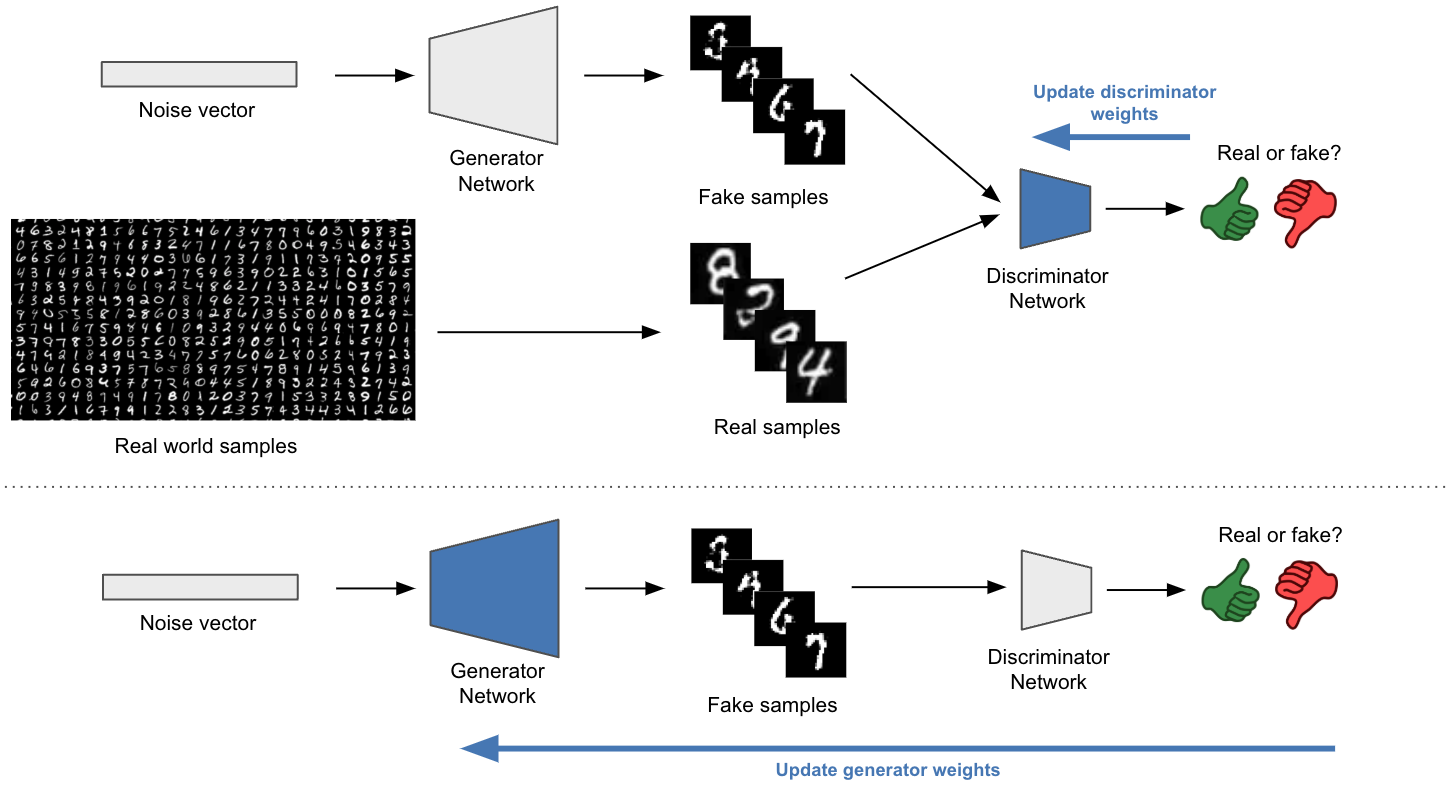
\includegraphics[width=0.90\columnwidth]{fig_datasynth/gans_training_shematic.png} 
    % \vspace{-2pt}
    % \caption{\label{fig:gans_schematic} GAN training framework. In stage one (top) the discriminator is trained and in stage two (bottom) the generator is trained. Blue color is used to represent the blocks being trained in each stage.}
    % \vskip -0.0in 
\end{figure}


The initial GAN-based models introduced in the MANOLO data synthesis module for class-conditional sample generation are the Conditional GAN (CGAN)~\citep{2014_arxiv_CGAN}, and the Deep Convolutional GAN (DCGAN)~\citep{2015_ICLR_DCGAN}. The first one is composed of linear components and is used for smaller datasets where the model easily captures the features of the data while the second one includes convolutions to address more complex data.
        
\subsubsection{Methodology}

This subsection introduces the methodology followed in this version of the deliverable to generate samples with GAN-based models conditioned to a particular class. The generator network in GANs learns to map an input noise vector in a fixed latent space to the sample space resulting in a newly generated sample. By concatenating a representation of the class label to the input noise vector, the generator network is conditioned to generate a sample belonging to a particular class. This label representation could be a one-hot-encoding of the label as done by Mirza and Osindero~\citep{2014_arxiv_CGAN} to condition the CGAN model, or more complex alternatives including linear or embedding layers, as we do in this version of the deliverable to condition the DCGAN model.


\subsubsection*{Experimental setup.} 
\begin{quote}
Following the methodology in Section~\ref{subsec:2.3_datasynth_tech1} we develop and test the CGAN model in MNIST and Fashion-MNIST. Additionally, to test the scalability capabilities of the GAN-framework we use CIFAR-10~\cite{2009_CIFAR} for the DCGAN model. CIFAR-10 is an RGB natural-images dataset with 60,000 32$\times$32 samples divided into 10 classes and split into a set for training with 50,000 samples and a set for testing with 10,000.

The CGAN model used in this section is constituted by a generator network with four linear layers followed by LeakyReLU non-linearity and a discriminator network with four linear layers followed by LeakyReLU non-linearity and dropout layers with a probability of 0.3. We use a 100-dimensions noise vector and condition the model by concatenating the noise vector to the one-hot-encoding of the labels. The DCGAN model, on the other hand, is constituted by a generator network with three transpose convolution layers followed by batch normalization and ReLU non-linearity layers and a last transpose convolution layer followed by a tanh non-linearity layer. Then the class conditioning is done by projecting the noise vector to a 7 $\times$ 7 $\times$ 128 dimension space and concatenating it to a 7 $\times$ 7 $\times$ 1 projection of a learned 50-dimensions embedding of the labels. This results in a 7 $\times$ 7 $\times$ 129 input vector for the generator. The discriminator, then, consist of four convolutional layers followed by batch normalization and LeakyReLU non-linearity layers, followed by a final linear layer and a sigmoid non-linearity layer. The conditioning of the discriminator is done in a similar fashion, where the labels are projected to a 32 $\times$ 32 $\times$ 1 space and concatenated to the input samples, both real and newly generated. Both models are trained with the Adam optimizer with learning rate of $10^{-4}$ on 128 samples batches for 200 epochs.
\end{quote}

\subsubsection{Results}

The results showed in this section illustrate the effectiveness of GAN to generate images. Figure~\ref{fig:cGAN_MNIST} and~\ref{fig:cGAN_FashionMNIST} provide images generated with a CGAN for MNIST and Fashion-MNIST respectively. This visualization show that the model successfully generate images according to the specified class. We also notice that the quality of the images is still lower than the quality of the real images found in the dataset, this could be improved with further exploration of the hyperparamter space (e.g. larger training time or deeper models or different optimization strategies). Then, Figure~\ref{fig:DCGAN_CIFAR10} provides images generated with the DCGAN model for the CIFAR-10 dataset. These images also show how the generator of the DCGAN captures the general distribution of the data and is able to reproduce CIFAR-10-like images. Note that, when examined in more detail, these images depict parts of objects and realistic shapes that resemble visual features present in the original dataset.


\begin{figure}
    % \vskip -0.2in 
    \centering
    \caption{\label{fig:cGAN_MNIST} Samples generated by the CGAN for each of the ten classes in the MNIST dataset.}
    \vspace{-0.1in}
    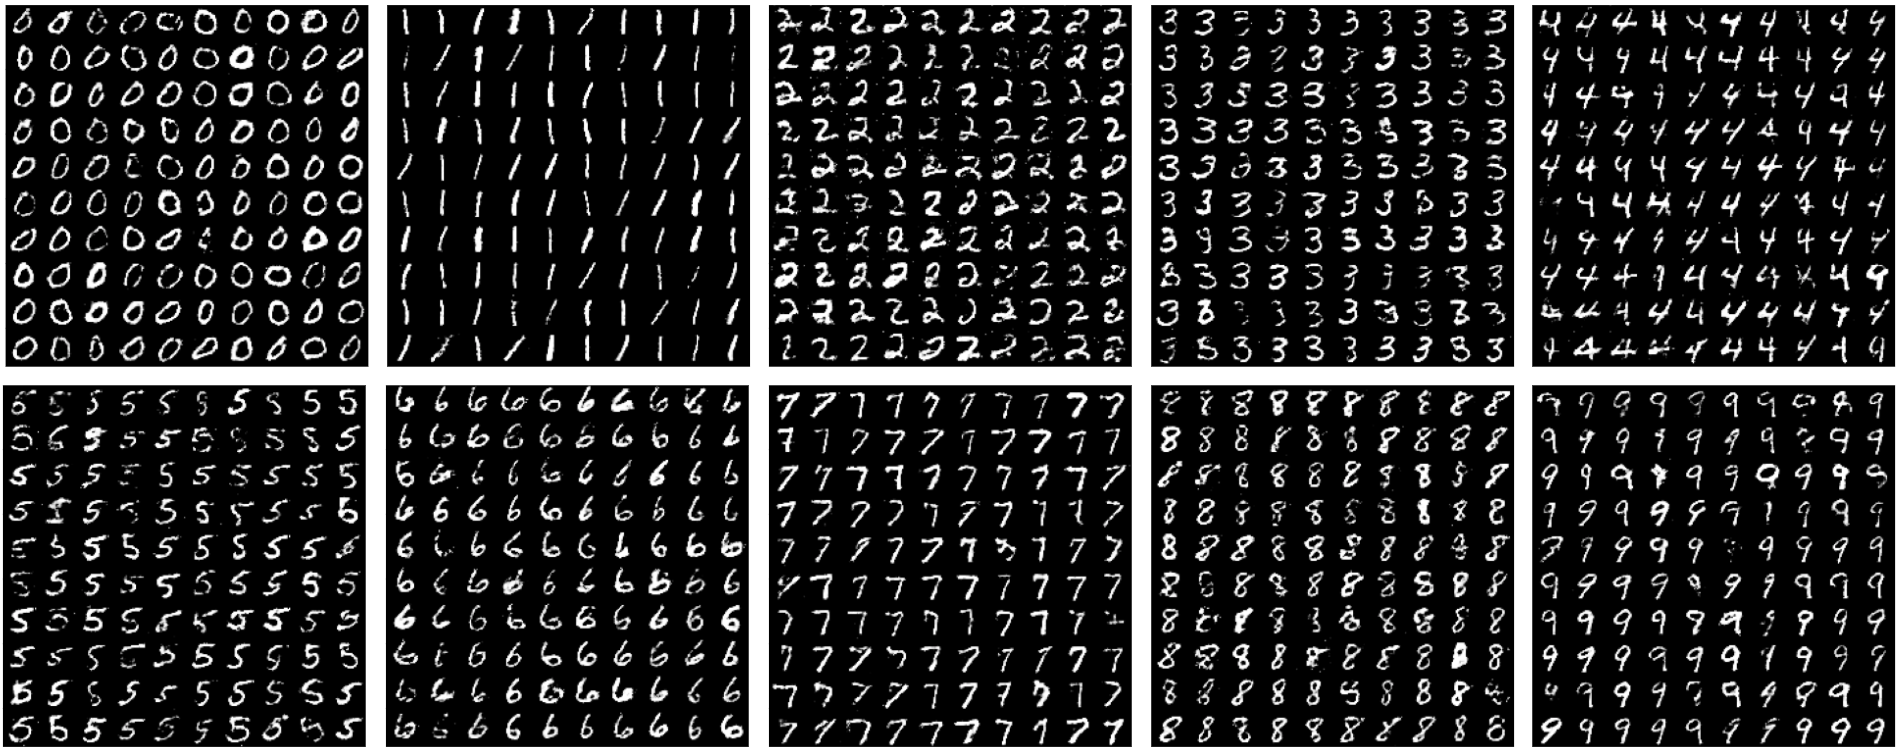
\includegraphics[width=0.95\columnwidth]{fig_datasynth/mnist_cGANs.png} 
    % \vspace{-0.1in}
    % \caption{\label{fig:cGAN_MNIST} Samples generated by the CGAN for each of the ten classes in the MNIST dataset.}
    % \vskip -0.0in 
\end{figure}

\begin{figure}
    % \vskip -0.2in 
    \centering
    \caption{\label{fig:cGAN_FashionMNIST} Samples generated by the CGAN for each of the ten classes in the Fashion-MNIST dataset.}
    \vspace{-0.1in}
    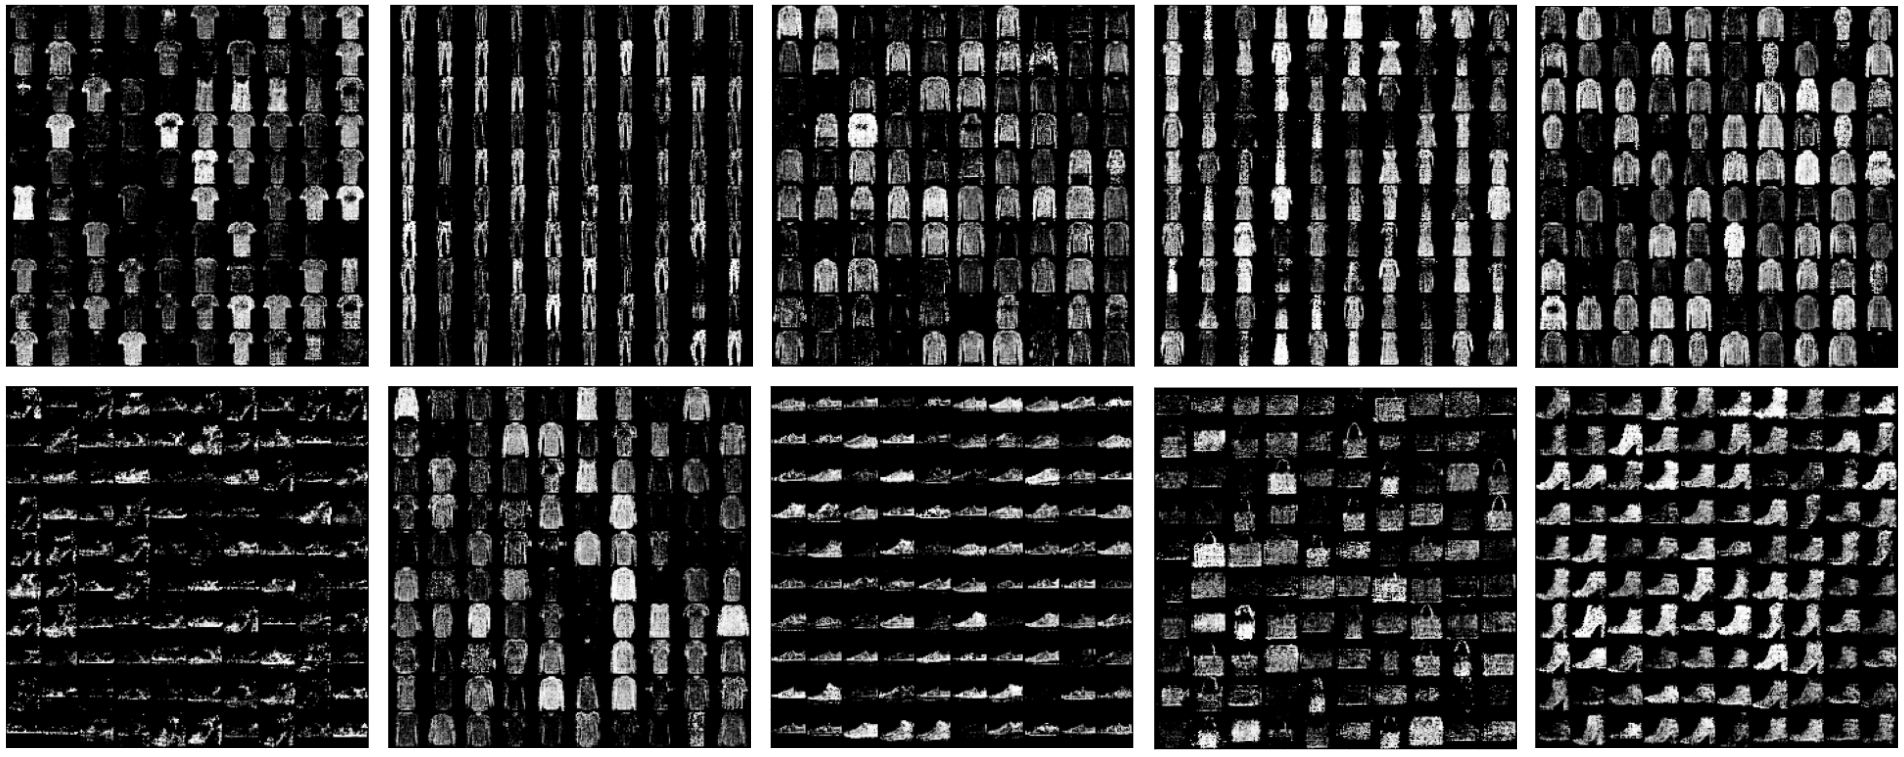
\includegraphics[width=0.95\columnwidth]{fig_datasynth/fashion-mnist_cGANs.png}     
    % \vspace{-0.1in}
    % \caption{\label{fig:cGAN_FashionMNIST} Samples generated by the CGAN for each of the ten classes in the Fashion-MNIST dataset.}
    % \vskip -0.0in 
\end{figure}    


\begin{figure}
    % \vskip -0.2in 
    \centering
    \caption{\label{fig:DCGAN_CIFAR10} Samples generated by the CDGAN for each of the ten classes in the CIFAR-10 dataset.}
    \vspace{-0.1in}
    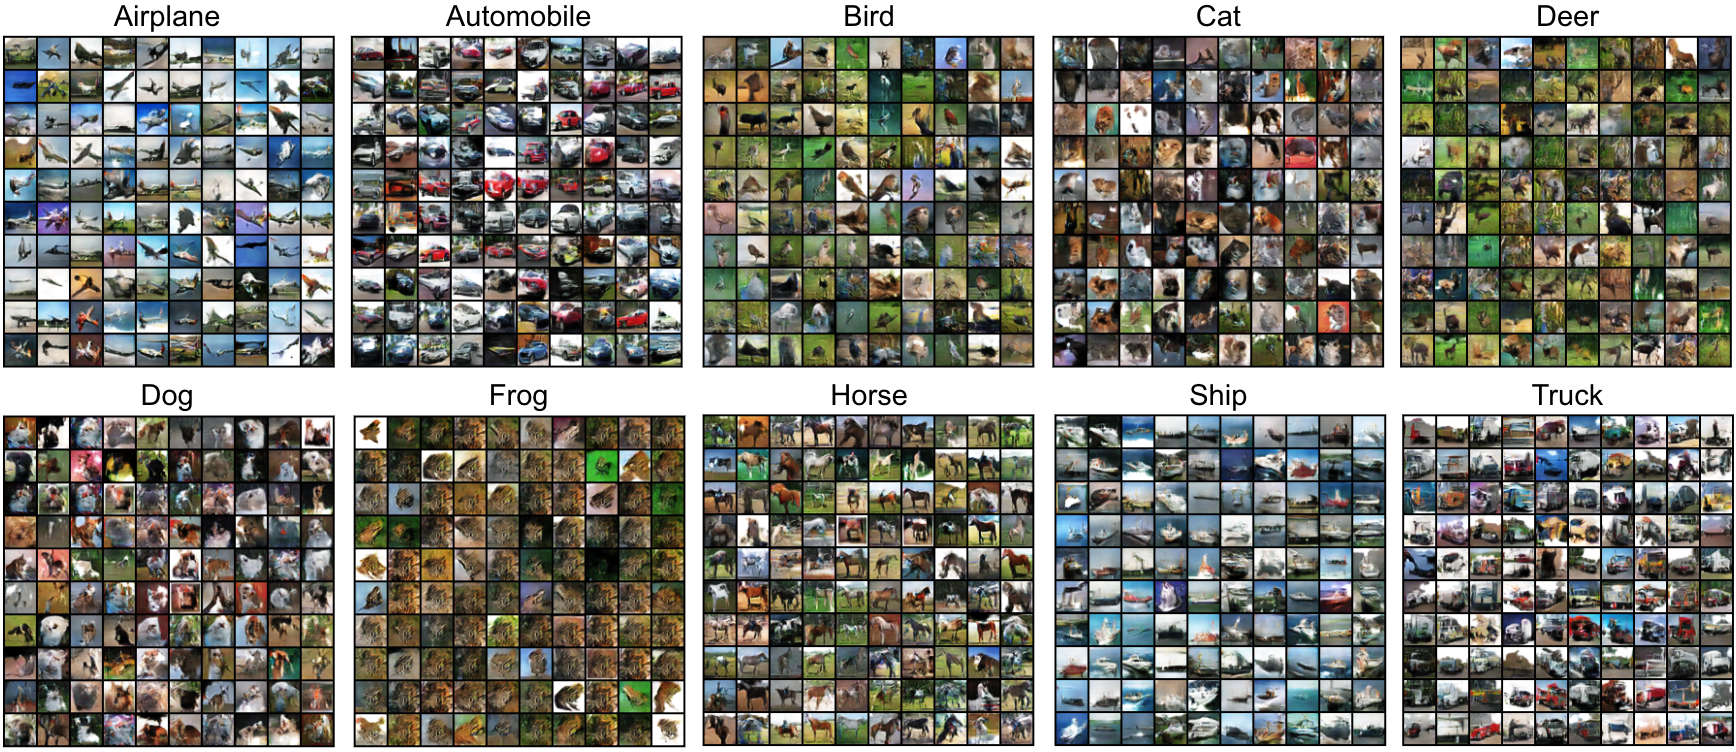
\includegraphics[width=0.95\columnwidth]{fig_datasynth/cifar_cond_DCGAN_large_softLab.png}     
    % \vspace{-0.1in}
    % \caption{\label{fig:DCGAN_CIFAR10} Samples generated by the CDGAN for each of the ten classes in the CIFAR-10 dataset.}
    % \vskip -0.0in 
\end{figure}    
